

\documentclass{beamer}

\mode<presentation> {

% The Beamer class comes with a number of default slide themes
% which change the colors and layouts of slides. Below this is a list
% of all the themes, uncomment each in turn to see what they look like.


\usetheme{Boadilla}



\setbeamertemplate{footline}  


}
\setbeamersize{text margin left=1cm, }
\setbeamertemplate{frametitle}[default][center]
\usepackage{graphicx} 
\usepackage{booktabs} 

	\usepackage{changepage}


\usepackage{cite}
\usepackage{setspace}
\usepackage{color}
\usepackage[normalem]{ulem}
\newtheorem{hyp}{Hypothesis}


\usepackage{epsfig}
\usepackage{amsmath}
\usepackage{amssymb}
\usepackage{multicol}
\usepackage{amsmath, amsthm, amssymb}


\usepackage{graphicx}
\usepackage{tikz}
\usetikzlibrary{shapes,arrows}
\usepackage{tikz}
\usepackage{amsmath, amsthm, amssymb}
%----------------------------------------------------------------------------------------
%	TITLE PAGE
%----------------------------------------------------------------------------------------



\begin{document}
	

  

\begin{frame}
	\frametitle{Web Data -- Scraping and APIs}

\end{frame}


\begin{frame}
	
	\centering\Huge{Scraping the web}
	
	
\end{frame}



\begin{frame}
	\frametitle{Scraping the web: what?}
	
	An increasing amount of data is available on the web:
	
	\begin{itemize}[<+->]
		\item Speeches, sentences, biographical information...
		\item Social media data, newspaper articles, press releases...
		\item Geographic information, conflict data...
	\end{itemize} 
	\onslide<+->
	\vspace{.25cm}
	These datasets are often provided in an \alert{unstructured format}. \\
	\onslide<+->
	\vspace{.25cm}
	\alert{Web scraping} is the process of extracting this information automatically and transforming it into a \alert{structured dataset.}
	
\end{frame}

\begin{frame}
	\frametitle{Scraping the web: why?}
	
	\begin{itemize}[<+->]
		\item Copy \& pasting is time-consuming, boring, prone to errors, and impractical for large datasets
		\item In contrast, automated web scraping:
		\begin{enumerate}
			\item Scales well for large datasets
			\item Is reproducible
			\item Involved adaptable techniques
			\item Facilitates detecting and fixing errors
		\end{enumerate}
		\item When to scrape? 
		\begin{enumerate}
			\item Trade-off between your time today and your time in the future. \alert{Invest in your future self!}
			\item Computer time is cheap; human time is expensive
		\end{enumerate}
	\end{itemize}
	
\end{frame}

\begin{frame}
	\frametitle{Scraping the web: two approaches}
	
	Two different approaches:
	\vspace{.25cm}
	\begin{enumerate}[<+->]
		\item \alert{Screen scraping}: extract data from source code of website, with html parser and/or regular expressions
		\begin{itemize}
			\item \texttt{rvest} package in R
		\end{itemize}
		\vspace{.25cm}
		\item \alert{Web APIs }(application programming interfaces): a set of structured http requests that return JSON or XML data
		\begin{itemize}
			\item \texttt{httr} package to construct API requests
			\item Packages specific to each API:  \href{https://cran.r-project.org/web/packages/weatherData/index.html}{weatherData}, \href{https://cran.r-project.org/web/packages/WDI/index.html}{WDI}, \href{https://cran.r-project.org/web/packages/Rfacebook/index.html}{Rfacebook}... Check CRAN Task View on \href{https://cran.r-project.org/web/views/WebTechnologies.html}{Web Technologies and Services} for examples

		\end{itemize}
	\end{enumerate}
\end{frame}

\begin{frame}
	\frametitle{The rules of the game}
	
	\begin{enumerate}[<+->]
		\item Respect the hosting site's wishes:
		\begin{itemize}
			\item Check if an API exists or if data are available for download
			\item Keep in mind where data comes from and give credit (and respect copyright if you want to republish the data!)
			\item Some websites \textit{disallow} scrapers on \texttt{robots.txt} file
		\end{itemize}
		\vspace{.25cm}
		\item Limit your bandwidth use:
		\begin{itemize}
			\item Wait one or two seconds after each hit
			\item Scrape only what you need, and just once (e.g. store the html file in disk, and then parse it)
		\end{itemize}
		\vspace{.25cm}
		\item When using APIs, read documentation
		\begin{itemize}
			\item Is there a batch download option?
			\item Are there any rate limits?
			\item Can you share the data?
		\end{itemize}
	\end{enumerate}
\end{frame}

\begin{frame}
	\frametitle{The art of web scraping}
	
	Workflow:
	
	\begin{enumerate}[<+->]
		\item Learn about structure of website
		\item Choose your strategy
		\item Build prototype code: extract, prepare, validate
		\item Generalize: functions, loops, debugging
		\item Data cleaning
	\end{enumerate}
	
\end{frame}

\begin{frame}
	\frametitle{The art of web scraping}
	\centering
	
\includegraphics[width=1\textwidth]{figures/whattouse.jpg}
	
	\Large{\alert{Three main scenarios}}
	
\end{frame}

\begin{frame}
	\frametitle{Three main scenarios}
	
	1. Data in table format \\
	\vspace{.25cm}
	
	
	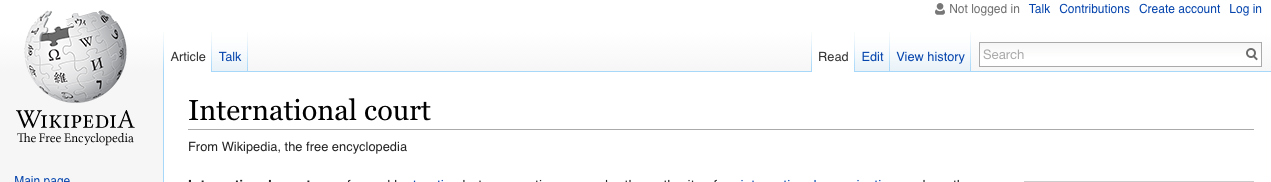
\includegraphics[width=1\textwidth]{figures/wikitable1.png}\\
	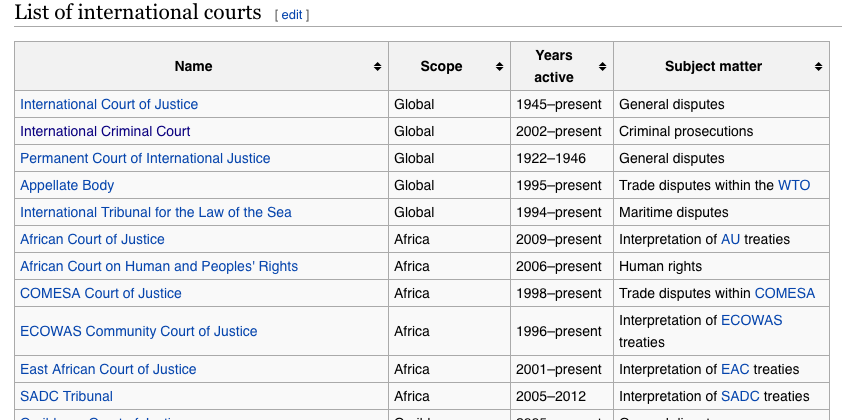
\includegraphics[width=\textwidth]{figures/wikitable2.png}
	
\end{frame}

\begin{frame}
	\frametitle{Three main scenarios}
	
	2. Data in unstructured format  \\
	\vspace{.25cm}
	
	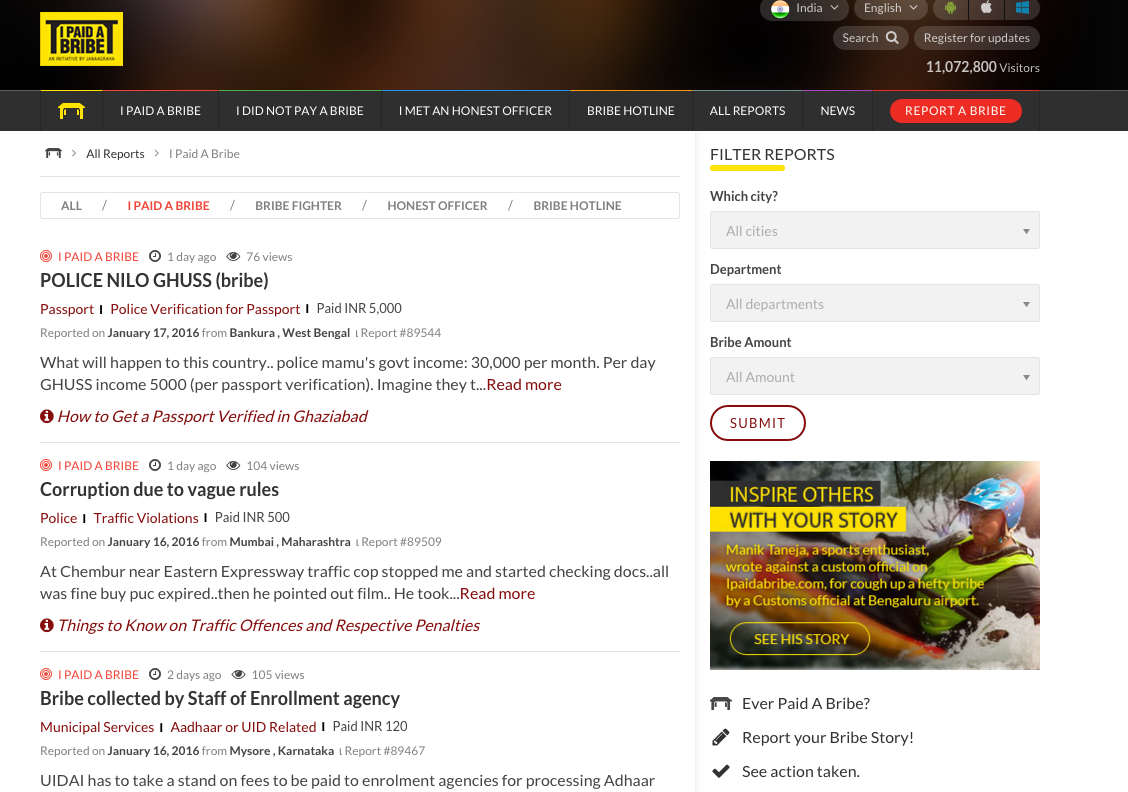
\includegraphics[width=.9\textwidth]{figures/bribe.png}
	
	\centering\href{www.ipaidabribe.com/reports/paid}{www.ipaidabribe.com/reports/paid}
\end{frame}

\begin{frame}
	\frametitle{Three main scenarios}
	
	3. Data hidden behind web forms \\
	\vspace{.25cm}
	
	
	\includegraphics[width=\textwidth]{figures/Venezuela.png}
	
	\centering\href{http://eligetucandidato.org/filtro/}{Candidates on 2015 Venezuelan parliamentary election}
\end{frame}

\begin{frame}
	\frametitle{Three main scenarios}
	
	\begin{enumerate}[<+->]
		
		\item Data in \alert{table} format
		\begin{itemize}
			\item Automatic extraction with \texttt{rvest}
		\end{itemize}
		\vspace{.25cm}
		\item Data in \alert{unstructured} format
		\begin{itemize}
			\item Element identification with \texttt{selectorGadget}
			\item Automatic extraction with \texttt{rvest}
		\end{itemize}
		\vspace{.25cm}
	
		
	\end{enumerate}
	
\end{frame}

\begin{frame}[fragile]
	\frametitle{HTML: a primer}
	Hypertext Markup Language (HTML): hidden standard behind every website. \pause
	\begin{itemize}
		\item HTML is text with marked-up structure, defined by \alert{tags}:
		\item\begin{verbatim}
		<!DOCTYPE html>
		<html>
		<body>
		
		<h1>My First Heading</h1>
		
		<p>My first paragraph.</p>
		
		</body>
		</html>
		\end{verbatim}
		\item What you see in your browser is an interpretation of the HTML document
	\end{itemize}
	
\end{frame}

\begin{frame}[fragile]
	\frametitle{HTML: a primer}
	\begin{itemize}[<+->]
		\item Some common tags:
		\begin{itemize}
			\item Document elements: \verb|<head>|, \verb|<body>|, \verb|<footer>|...
			\item Document components: \verb|<title>|,\verb|<h1>|, \verb|<div>|...
			\item Text style: \verb|<b>|, \verb|<i>|, \verb|<strong>|...
			\item Hyperlinks: \verb|<a>|
		\end{itemize}
		\item  An example: \href{http://www.pablobarbera.com}{www.pablobarbera.com}
	\end{itemize}
\end{frame}


\begin{frame}[fragile]
	\frametitle{Beyond HTML}
	
	\begin{itemize}
		\item \alert{Cascading Style Sheets} (CSS): describes formatting of HTML components (e.g. \verb|<h1>|, \verb|<div>|...), useful for us!
		
		\begin{center} 
\includegraphics[width=.5\textwidth]{figures/htmlcss.jpg} \end{center}
		
		\item \alert{Javascript}: adds functionalities to the website (e.g. change content/structure after website has been loaded)
	\end{itemize}
	
\end{frame}

\begin{frame}
	\frametitle{Parsing HTML code}
	
	First step in webscraping: read HTML code in R and \alert{parse it} \pause
	\begin{itemize}[<+->]
		\item Parsing = understanding structure
		\item How? \texttt{rvest} package in R:
		\begin{itemize}
			\item \texttt{read\_html}: parse HTML code into R
			\item \texttt{html\_text}: extract text from HTML code
			\item \texttt{html\_table}: extract tables in HTML code
			\item \texttt{html\_nodes}: extract components with CSS selector 
			\item \texttt{html\_attrs}: extract attributes of nodes
		\end{itemize}
		\item How to identify relevant CSS selectors? \texttt{selectorGadget} extension for Chrome and Firefox.
	\end{itemize}
	
	
\end{frame}



\begin{frame}
	
	\centering\Huge{APIs}
	
\end{frame}



\begin{frame}
	\frametitle{APIs}
	
	API = Application Programming Interface; a set of structured http requests that return data in a lightweight format.\\
	\vspace{.25cm}
	\pause
	HTTP = Hypertext Transfer Protocol; how browsers and e-mail clients communicate with servers.\\
	\vspace{.20cm}
	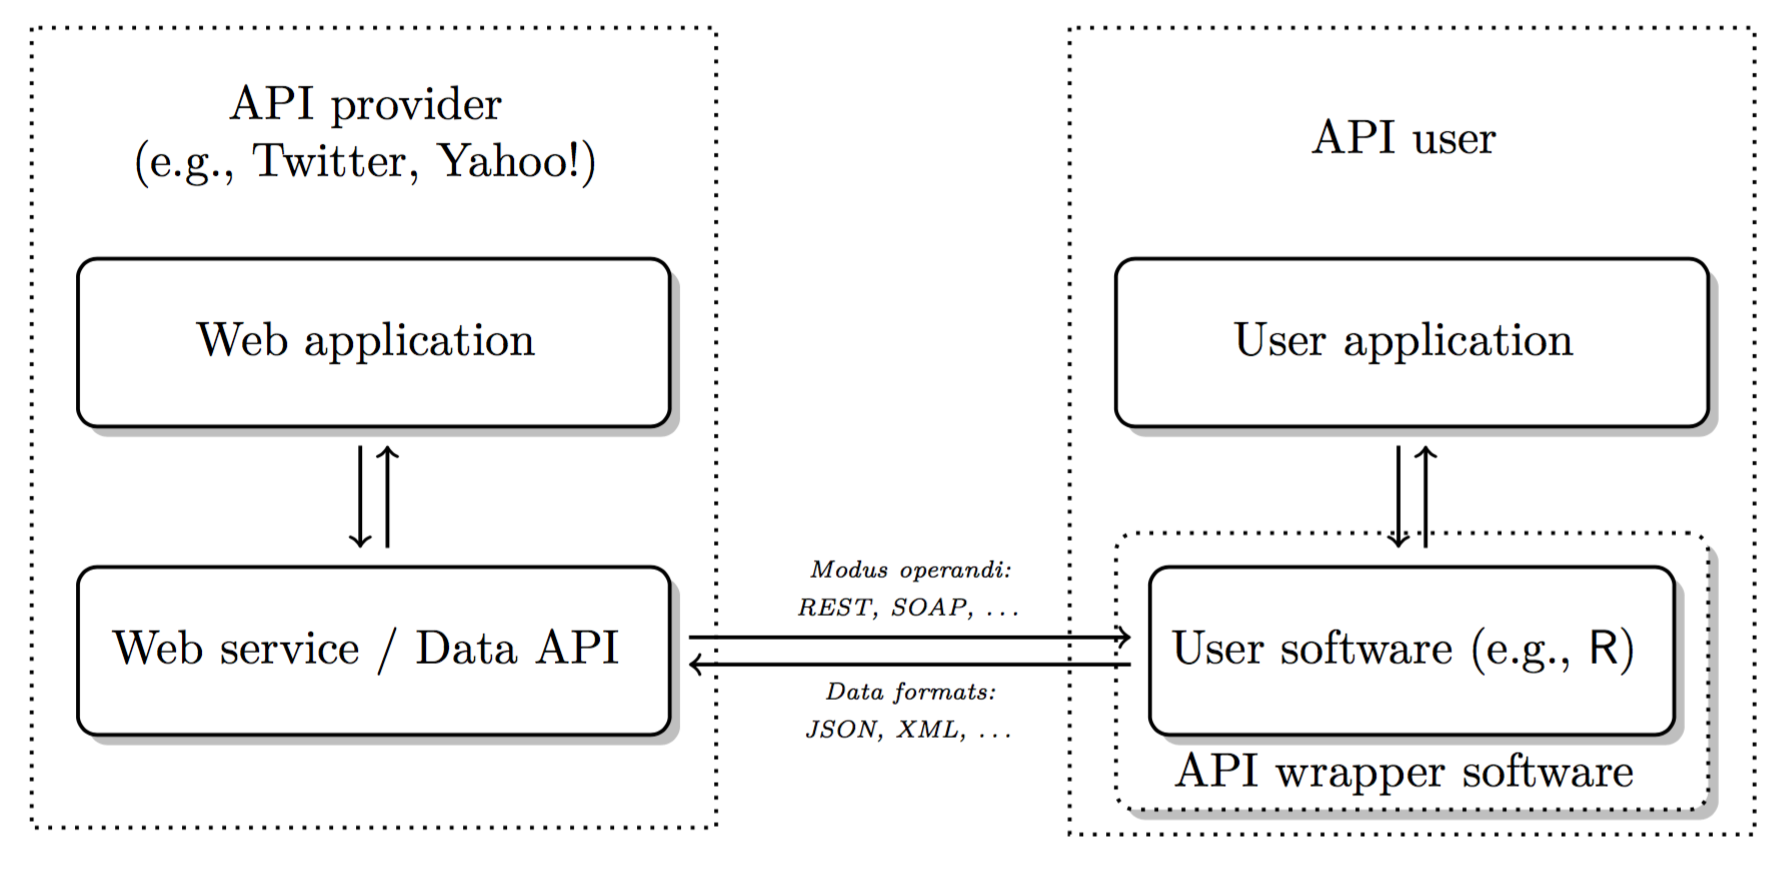
\includegraphics[width=.9\textwidth]{figures/apis.png} \\
	\hfill\small{\textbf{Source}: Munzert et al, 2014, Figure 9.8}
	
	
\end{frame}

\begin{frame}
	\frametitle{APIs}
	Types of APIs:  
	\begin{enumerate}
		\item \alert{RESTful APIs}: queries for static information at current moment (e.g. user profiles, posts, etc.)  
		\item \alert{Streaming APIs}: changes in users' data in real time (e.g. new tweets, weather alerts...)  
	\end{enumerate}
	\pause
	\vspace{.10cm}
	APIs generally have extensive \alert{documentation}:
	\begin{itemize}
		\item Written for developers, so must be understandable for humans
		\item What to look for: \alert{endpoints} and \alert{parameters.}
	\end{itemize}
	\pause
	\vspace{.10cm}
	Most APIs are \alert{rate-limited:}
	\begin{itemize}
		\item Restrictions on number of API calls by user/IP address and period of time.
		\item Commercial APIs may impose a monthly fee
	\end{itemize}
\end{frame}

\begin{frame}[fragile]
	\frametitle{Connecting with an API}
	
	Constructing a REST API call:
	\vspace{.20cm}
	\begin{itemize}
		\item Baseline URL \alert{endpoint}: \scriptsize{\texttt{https://maps.googleapis.com/maps/api/geocode/json}}
		\item Parameters: \texttt{?address=budapest}
		\item Authentication token (optional): \texttt{\&key=XXXXX}
	\end{itemize}
	\vspace{.20cm}
	From R, use \texttt{httr} package to make \texttt{GET} request:\\
	\vspace{.10cm}
	\begin{small}
		\begin{verbatim}
		library(httr)
		r <- GET(
		"https://maps.googleapis.com/maps/api/geocode/json",
		query=list(address="budapest"))
		\end{verbatim}
	\end{small}
	If request was successful, returned code will be \texttt{200}, where \texttt{4xx} indicates client errors and \texttt{5xx} indicates server errors.\\
	If you need to attach data, use \texttt{POST} request.
	
\end{frame}


\begin{frame}[fragile]
	\frametitle{JSON}
	Response is often in \href{https://maps.googleapis.com/maps/api/geocode/json?address=budapest}{JSON format} (Javascript Object Notation). \\ \pause
	\begin{itemize}[<+->]
		\item Type: \verb|content(r, "text")|
		\item Data stored in key-value pairs. Why? Lightweight, more flexible than traditional table format.
		\item Curly brackets embrace objets; square brackets enclose arrays (vectors)
		\item Use \texttt{fromJSON} function from \texttt{jsonlite} package to read JSON data into R
		\item But many packages have their own specific functions to read data in JSON format; \verb|content(r, "parsed")|
	\end{itemize}
	
	
	
\end{frame}

\begin{frame}
	\frametitle{Authentication}
	\begin{itemize}
		\item Many APIs require an access key or token
		\item An alternative, open standard is called OAuth  
		\item Connections without sharing username or password, only temporary tokens that can be refreshed  
		\item \texttt{httr} package in R implements most cases (\href{https://github.com/hadley/httr/tree/master/demo}{examples})
	\end{itemize}
\end{frame}

\begin{frame}
	\frametitle{R packages}
	
	Before starting a new project, worth checking if there's already an R package for that API. Where to look?
	\begin{itemize}
		\item \href{https://cran.r-project.org/web/views/WebTechnologies.html}{CRAN Web Technologies Task View} (but only packages released in CRAN)
		\item GitHub (including unreleased packages and most recent versions of packages)
		\item \href{https://ropensci.org/}{rOpenSci Consortium}
		
	\end{itemize}
	
	\uncover<+->{Also see this \href{https://github.com/toddmotto/public-apis}{great list of APIs} in case you need inspiration}.
	
\end{frame}

\begin{frame}
	\frametitle{Why APIs?}
	
	\alert{Advantages}:
	\begin{itemize}[<+->]
		\item `Pure' data collection: avoid malformed HTML, no legal issues, clear data structures, more trust in data collection...
		\item Standardized data access procedures: transparency, replicability
		\item Robustness: benefits from `wisdom of the crowds'
	\end{itemize}
	\uncover<+->{\alert{Disadvantages}}
	\begin{itemize}[<+->]
		\item They're not too common (yet!)
		\item Dependency on API providers
		\item Lack of natural connection to R
	\end{itemize}
	
\end{frame}




\end{document} 